
\section{Liniowa teoria sprężystości}
\label{sec:liniowa_teoria_sprezystosci}

Liniowa teoria sprężystości jest mechaniką ciała stałego opartą na następujących założeniach:
\begin{itemize}
  \item ciało jest wypełnione materią w sposób ciągły zarówno przed jak i po odkształceniu
  \item odkształcenia i przemieszczenia są bardzo małe
  \item spełniona jest zasada superpozycji
  \item ośrodek zachowuje się zgodnie z prawem Hooke'a
  \item siły działają na ciało w taki sam sposób przed odkształeceniem jak i po odkształceniu
\end{itemize}

\subsection{Naprężenie}
\label{sec:naprezenie}

Naprężenie można zdefiniować jako miara sił wewnętrznych ciała w punkcie. Weźmy ciało przedstawione na rysunku \ref{fig:potato}, na które działają siły zewnętrzne P1 i P2. W płaszczyźnie przekroju wybieramy punkt B, w którego otoczeniu określamy pole dA. Stosunek sił jakimi oddziałują na siebie połówki ciała w tym punkcie przekroju, do pola dA, nazywamy naprężeniem ciała w punkcie B. Kierunek naprężenia będzie zgodny z kierunkiem działania siły przekrojowej w punkcie.

\begin{figure}[h]
\centering
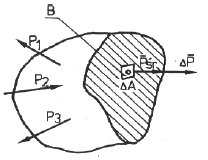
\includegraphics[width=5cm]{Zdjecia/2/potato}
\caption{Ciało pod wpływem sił zewnętrznych}
\label{fig:potato}
\end{figure}

Stana naprężenia w punkcie B oznacza ogół naprężeń, które otrzymamy dla wszystkich możliwych przekrojów ciała przez ten punkt.
W przypadku trójwymiarowego stanu naprężenia, dla każdego przekroju wektor naprężenia będzie miał inny kierunek. Stan naprężenia można opisać przy pomocy tensora naprężeń, dla układu kartezjańskiego danego wzorem:


\begin{gather}
	\sigma=\begin{bmatrix} 
	  \sigma_{xx}    & \tau_{xy} & \tau_{xz} \\ 
	  \tau_{yx} & \sigma_{yy} & \tau_{yz} \\
	  \tau_{zx} & \tau_{zy} & \sigma_{zz} 
	\end{bmatrix}
\end{gather}

gdzie

\begin{eqwhere}[2cm]
        \item[$\sigma_{ii}$] naprężenie normalne, i=(x, y, z)
        \item[$\tau_{ij}$] naprężenie styczne, i,j=(x, y, z), \( i \neq j, \tau_{ij}=\tau_{ji}\)
\end{eqwhere}

\subsection{Odkształcenie i prawko Hooke'a}
\label{sec:odksztalcenie_i_prawo_hookea}

	Pod wpływem naprężeń ciało sprężyste ulega odkształceniu. Możemy wyróżnić odkształcenia liniowe \( \varepsilon_i \) oraz odkształcenia postaciowe \( \gamma_{ij} \). Najprostszym przypadkiem odkształcenia liniowego jest rozciąganie pręta. Poniżej znajduje się rysunek pręta rozciąganego siłą P. 

\begin{figure}[h]
\centering
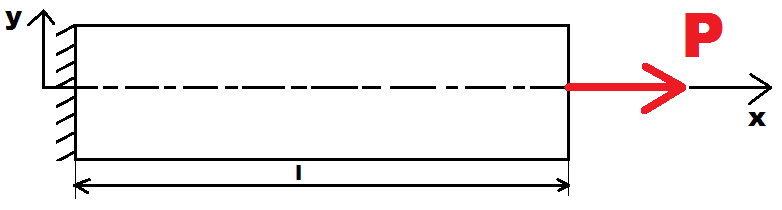
\includegraphics[width=10cm]{Zdjecia/2/rozciaganie}
\caption{Rozciąganie pręta}
\label{fig:rozciaganie}
\end{figure}

	W takim przypadku odkształceniem wzdłużnym będziemy nazywać stosunek wydłużenia pręta do jego początkowej długości:

\begin{equation}
\varepsilon_x=\frac{\Delta l}{l}.
\end{equation}
	
	Odkształceniem poprzecznym(postaciowym) nazywać będziemy stosunek zmiany średnicy przekroju do jego początkowej średnicy:

\begin{equation}
\varepsilon_y=\frac{\Delta d}{d}.
\end{equation}

	Odkształcenia te związane są zależnością:

\begin{equation}
\varepsilon_x=-\nu \varepsilon_y
\end{equation}
gdzie
\begin{eqwhere}[2cm]
        \item[$\nu$] współczynnik Poissona.
\end{eqwhere}

	Współczynnik Poissona jest wielkością bezwymiarową. Określa on sposób w jaki odkształca się ciało i przyjmuje wartości z przedziału [-1, 1]. Dla popularnych w mechanice stopów metali przyjmuje zwykle wartości z przedziału [0.2 , 0.4]. Wartości ujemne przyjmuje dla tak zwanych materiałów odwrotnych, które pod wpływem naprężenia zwiększają swoją objętość.

	Dla przypadku prostego rozciągania zachodzi jeszcze jedna zależność. Opisuje ona związek pomiędzy naprężeniem i odkształceniem i nazywana jest prawem Hooke'a.

\begin{equation}
\sigma=E\varepsilon
\end{equation}
gdzie
\begin{eqwhere}[2cm]
        \item[$E$] moduł Younga.
\end{eqwhere}

	Moduł Younga określa zależność odkształcenia liniowego i przyłożonego naprężenia. Jednostką moduły Younga jest paskal, a wartości podaje się w gigapasklach (GPa). Wartości dla stali wynoszą około 200 GPa, a dla aluminium około 70 GPa.

	W przypadku trójwymiarowego rozkładu okształceń stosuje się zapis tensorowy. Tensor odkształcenia znajduje się poniżej:
\begin{gather}
	\varepsilon=\begin{bmatrix} 
	  \varepsilon_{xx}    & \gamma_{xy} & \gamma_{xz} \\ 
	  \gamma_{yx} & \varepsilon_{yy} & \gamma_{yz} \\
	  \gamma_{zx} & \gamma_{zy} & \varepsilon_{zz} 
	\end{bmatrix}
\end{gather}

%\[
%	\textbf{$\varepsilon$}=\begin{bmatrix} 
%	  \varepsilon_{xx}    & \gamma_{xy} & \gamma_{xz} \\ 
%	  \gamma_{yx} & \varepsilon_{yy} & \gamma_{yz} \\
%	  \gamma_{zx} & \gamma_{zy} & \varepsilon_{zz} 
%	\end{bmatrix}
%\]

gdzie

\begin{eqwhere}[2cm]
        \item[$\varepsilon_{ii}$] odkształcenie liniowe, i=(x, y, z)
        \item[$\gamma_{ij}$] odkształcenie postaciowe, i,j=(x, y, z), \( i \neq j, \tau_{ij}=\tau_{ji}\)
\end{eqwhere}

Dla takiego przypadku prawo Hooke'a przybiera bardziej skomplikowaną postać:

\begin{equation}
\varepsilon_xx=\frac{1}{E}(\sigma_xx-\nu(\sigma_yy+\sigma_zz)), \gamma_{xy}=\frac{\tau_{xy}}{G}
\end{equation}
\begin{equation}
\varepsilon_yy=\frac{1}{E}(\sigma_yy-\nu(\sigma_xx+\sigma_zz)), \gamma_{xz}=\frac{\tau_{xz}}{G}
\end{equation}
\begin{equation}
\varepsilon_zz=\frac{1}{E}(\sigma_zz-\nu(\sigma_xx+\sigma_yy)), \gamma_{yz}=\frac{\tau_{yz}}{G}
\end{equation}

\begin{eqwhere}[2cm]
        \item[$G$] moduł Kirchoffa
\end{eqwhere}

	Moduł Kirchoffa opisuje zależność odkształcenia postaciowego od naprężenia stycznego występującego w materiale. Jednostką tego współczynnika jest paskal, a typowymi wartościami są dla stali 80 Gpa, dla aluminium 25,5 GPa.

	Opisane wcześniej stałe materiałowe są powiązane równaniem:
\begin{equation}
E=2G(\nu+1)
\end{equation}

%\begin{equation}
%c_L=\sqrt{\frac{\lambda+2\mu}{\rho}}
%\end{equation}
%gdzie
%\begin{eqwhere}[2cm]
%        \item[$c_L$] prędkość fali podłużnej
%        \item[$\lambda, \mu$] stałe Lam\'{e}go
%        \item[$\rho$] gęstość ośrodka
%\end{eqwhere}
%
%\begin{figure}[h]
%\centering
%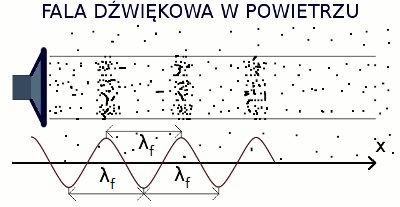
\includegraphics[width=10cm]{Zdjecia/2/fala_podluzna}
%\caption{Przykład fali podłużnej}
%\label{fig:fala_podluzna}
%\end{figure}
%
%
%
%\begin{figure}[h]
%        \centering
%        \begin{subfigure}{0.35\textwidth}
%                \centering
%	     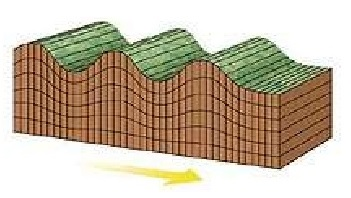
\includegraphics[width=5cm]{Zdjecia/2/fala_rayleigha}
%                \subcaption{\label{subfigure_a}}
%        \end{subfigure}
%        \begin{subfigure}{0.35\textwidth}
%                \centering
%	     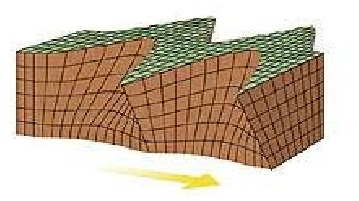
\includegraphics[width=5cm]{Zdjecia/2/fala_lova}
%                \subcaption{\label{subfigure_b}}
%        \end{subfigure}
%        \label{fig:subcaption_example}
%        \caption{Fale powierzchniowe: \protect\subref{subfigure_a} fala Rayleigha, \protect\subref{subfigure_b} fala L\"{o}va}
%\end{figure}





















